
% LaTeX Beamer file automatically generated from DocOnce
% https://github.com/hplgit/doconce

%-------------------- begin beamer-specific preamble ----------------------

\documentclass{beamer}

\usetheme{red_shadow}
\usecolortheme{default}

% turn off the almost invisible, yet disturbing, navigation symbols:
\setbeamertemplate{navigation symbols}{}

% Examples on customization:
%\usecolortheme[named=RawSienna]{structure}
%\usetheme[height=7mm]{Rochester}
%\setbeamerfont{frametitle}{family=\rmfamily,shape=\itshape}
%\setbeamertemplate{items}[ball]
%\setbeamertemplate{blocks}[rounded][shadow=true]
%\useoutertheme{infolines}
%
%\usefonttheme{}
%\useinntertheme{}
%
%\setbeameroption{show notes}
%\setbeameroption{show notes on second screen=right}

% fine for B/W printing:
%\usecolortheme{seahorse}

\usepackage{pgf}
\usepackage{graphicx}
\usepackage{epsfig}
\usepackage{relsize}

\usepackage{fancybox}  % make sure fancybox is loaded before fancyvrb

\usepackage{fancyvrb}
\usepackage{minted} % requires pygments and latex -shell-escape filename
%\usepackage{anslistings}
%\usepackage{listingsutf8}

\usepackage{amsmath,amssymb,bm}
%\usepackage[latin1]{inputenc}
\usepackage[T1]{fontenc}
\usepackage[utf8]{inputenc}
\usepackage{colortbl}
\usepackage[english]{babel}
\usepackage{tikz}
\usepackage{framed}
% Use some nice templates
\beamertemplatetransparentcovereddynamic

% --- begin table of contents based on sections ---
% Delete this, if you do not want the table of contents to pop up at
% the beginning of each section:
% (Only section headings can enter the table of contents in Beamer
% slides generated from DocOnce source, while subsections are used
% for the title in ordinary slides.)
\AtBeginSection[]
{
  \begin{frame}<beamer>[plain]
  \frametitle{}
  %\frametitle{Outline}
  \tableofcontents[currentsection]
  \end{frame}
}
% --- end table of contents based on sections ---

% If you wish to uncover everything in a step-wise fashion, uncomment
% the following command:

%\beamerdefaultoverlayspecification{<+->}

\newcommand{\shortinlinecomment}[3]{\note{\textbf{#1}: #2}}
\newcommand{\longinlinecomment}[3]{\shortinlinecomment{#1}{#2}{#3}}

\definecolor{linkcolor}{rgb}{0,0,0.4}
\hypersetup{
    colorlinks=true,
    linkcolor=linkcolor,
    urlcolor=linkcolor,
    pdfmenubar=true,
    pdftoolbar=true,
    bookmarksdepth=3
    }
\setlength{\parskip}{7pt}  % {1em}

\newenvironment{doconceexercise}{}{}
\newcounter{doconceexercisecounter}
\newenvironment{doconce:movie}{}{}
\newcounter{doconce:movie:counter}

\newcommand{\subex}[1]{\noindent\textbf{#1}}  % for subexercises: a), b), etc

%-------------------- end beamer-specific preamble ----------------------

% Add user's preamble




% insert custom LaTeX commands...

\raggedbottom
\makeindex

%-------------------- end preamble ----------------------

\begin{document}

% matching end for #ifdef PREAMBLE
% #endif

\newcommand{\half}{\frac{1}{2}}
\newcommand{\halfi}{{1/2}}
\newcommand{\tp}{\thinspace .}

\newcommand{\uex}{{u_{\small\mbox{e}}}}
\newcommand{\uexd}[1]{{u_{\small\mbox{e}, #1}}}
\newcommand{\vex}{{v_{\small\mbox{e}}}}
\newcommand{\vexd}[1]{{v_{\small\mbox{e}, #1}}}
\newcommand{\Aex}{{A_{\small\mbox{e}}}}

% Operators
\newcommand{\Ddt}[1]{\frac{D #1}{dt}}
\newcommand{\E}[1]{\hbox{E}\lbrack #1 \rbrack}
\newcommand{\Var}[1]{\hbox{Var}\lbrack #1 \rbrack}
\newcommand{\Std}[1]{\hbox{Std}\lbrack #1 \rbrack}

\newcommand{\xpoint}{\bm{x}}
\newcommand{\normalvec}{\bm{n}}
\newcommand{\Oof}[1]{\mathcal{O}(#1)}

% Boldface vectors/tensors
\newcommand{\x}{\bm{x}}
\newcommand{\X}{\bm{X}}
\renewcommand{\u}{\bm{u}}
\renewcommand{\v}{\bm{v}}
\newcommand{\w}{\bm{w}}
\newcommand{\acc}{\bm{a}}
\newcommand{\rpos}{\bm{r}}
\newcommand{\V}{\bm{V}}
\newcommand{\e}{\bm{e}}
\newcommand{\f}{\bm{f}}
\newcommand{\F}{\bm{F}}
\newcommand{\stress}{\bm{\sigma}}
\newcommand{\strain}{\bm{\varepsilon}}
\newcommand{\stressc}{{\sigma}}
\newcommand{\strainc}{{\varepsilon}}
\newcommand{\I}{\bm{I}}
\newcommand{\T}{\bm{T}}

\newcommand{\dfc}{\alpha}  % diffusion coefficient
% Unit vectors
\newcommand{\ii}{\bm{i}}
\newcommand{\jj}{\bm{j}}
\newcommand{\kk}{\bm{k}}
\newcommand{\ir}{\bm{i}_r}
\newcommand{\ith}{\bm{i}_{\theta}}
\newcommand{\iz}{\bm{i}_z}

% Index sets
\newcommand{\Ix}{\mathcal{I}_x}
\newcommand{\Iy}{\mathcal{I}_y}
\newcommand{\Iz}{\mathcal{I}_z}
\newcommand{\It}{\mathcal{I}_t}
%\newcommand{\Ix}{{I_x}}
%\newcommand{\Iy}{{I_y}}
%\newcommand{\Iz}{{I_z}}
%\newcommand{\It}{{I_t}}
%\newcommand{\If}{\mathcal{I}}     % for FEM
\newcommand{\If}{\mathcal{I}_s}     % for FEM
%\newcommand{\If}{{I}}     % for FEM
%\newcommand{\Ifd}{\mathcal{I}_d}  % for FEM
\newcommand{\Ifd}{{I_d}}  % for FEM
\newcommand{\Ifb}{{I_b}}  % for FEM
\newcommand{\setb}[1]{#1^0}    % set begin
\newcommand{\sete}[1]{#1^{-1}} % set end
%\newcommand{\setl}[1]{#1\setminus\{\set1{#1}\}}
%\newcommand{\setr}[1]{#1\setminus\{\set0{#1}\}}
%\newcommand{\seti}[1]{#1\setminus\{\set0{#1},\set1{#1}\}}
\newcommand{\setl}[1]{#1^-}
\newcommand{\setr}[1]{#1^+}
\newcommand{\seti}[1]{#1^i}
\newcommand{\sequencei}[1]{\left\{ {#1}_i \right\}_{i\in\If}}

% Finite elements
\newcommand{\basphi}{\varphi}
\newcommand{\baspsi}{\psi}
\newcommand{\refphi}{\tilde\basphi}
\newcommand{\psib}{\bm{\psi}}
\newcommand{\sinL}[1]{\sin\left((#1+1)\pi\frac{x}{L}\right)}
\newcommand{\xno}[1]{x_{#1}}
%\newcommand{\xno}[1]{x^{(#1)}}
\newcommand{\Xno}[1]{X_{(#1)}}
\newcommand{\yno}[1]{y_{#1}}
\newcommand{\Yno}[1]{Y_{(#1)}}
\newcommand{\xdno}[1]{\bm{x}_{#1}}

% FEniCS commands
\newcommand{\dX}{\, \mathrm{d}X}
\newcommand{\dx}{\, \mathrm{d}x}
\newcommand{\ds}{\, \mathrm{d}s}
\newcommand{\Real}{\mathbb{R}}
\newcommand{\Integerp}{\mathbb{N}}
\newcommand{\Integer}{\mathbb{Z}}



% ------------------- main content ----------------------



% ----------------- title -------------------------

\title{Study guide: Algorithms and implementations for exponential decay models}

% ----------------- author(s) -------------------------

\author{Hans Petter Langtangen\inst{1,2}}
\institute{Center for Biomedical Computing, Simula Research Laboratory\inst{1}
\and
Department of Informatics, University of Oslo\inst{2}}
% ----------------- end author(s) -------------------------

\date{Oct 17, 2015
% <optional titlepage figure>
% <optional copyright>
}

\begin{frame}[plain,fragile]
\titlepage
\end{frame}

\section{INF5620 in a nutshell}

\begin{frame}[plain,fragile]
\frametitle{INF5620 in a nutshell}

\label{5620:about}

\begin{itemize}
 \item Numerical methods for partial differential equations (PDEs)

 \item How do we solve a PDE in practice and produce numbers?

 \item How do we trust the answer?

 \item Approach: \emph{simplify, understand, generalize}
\end{itemize}

\noindent
\begin{block}{After the course }
You see a PDE and can't wait to program a method
and visualize a solution! Somebody asks if the solution is right
and you can give a convincing answer.
\end{block}


\end{frame}

\begin{frame}[plain,fragile]
\frametitle{The new official six-point course description}

After having completed INF5620 you

\begin{itemize}
\pause
 \item can derive methods and implement them to solve frequently
   arising partial differential equations (PDEs) from physics and mechanics.

\pause
 \item have a good understanding of finite difference and finite element
   methods and how they are applied in linear and nonlinear PDE problems.

\pause
 \item can identify numerical artifacts and perform mathematical analysis
   to understand and cure non-physical effects.

\pause
 \item can apply sophisticated programming techniques in Python, combined
   with Cython, C, C++, and Fortran code, to create modern,
   flexible simulation programs.

\pause
 \item can construct verification tests and automate them.

\pause
 \item have experience with project hosting sites (GitHub),
   version control systems (Git), report writing ({\LaTeX}),
   and Python scripting for performing reproducible computational science.
\end{itemize}

\noindent
\end{frame}

\begin{frame}[plain,fragile]
\frametitle{More specific contents: finite difference methods}

\begin{block}{}
\begin{itemize}
   \item ODEs

   \item the wave equation $u_{tt}=u_{xx}$ in 1D, 2D, 3D

   \item the diffusion equation $u_t=u_{xx}$ in 1D, 2D, 3D

   \item write your own software from scratch

   \item understand how the methods work and why they fail
\end{itemize}

\noindent
\end{block}
\end{frame}

\begin{frame}[plain,fragile]
\frametitle{More specific contents: finite element methods}

\begin{block}{}
\begin{itemize}
   \item stationary diffusion equations $u_{xx}=f$ in 1D

   \item time-dependent diffusion and wave equations in 1D

   \item PDEs in 2D and 3D by use of the FEniCS software

   \item perform hand-calculations, write your own software (1D)

   \item understand how the methods work and why they fail
\end{itemize}

\noindent
\end{block}
\end{frame}

\begin{frame}[plain,fragile]
\frametitle{More specific contents: nonlinear and advanced problems}

\begin{block}{}
\begin{itemize}
 \item Nonlinear PDEs
\begin{itemize}

   \item Newton and Picard iteration methods, finite differences and elements

\end{itemize}

\noindent
 \item More advanced PDEs for fluid flow and elasticity

 \item Parallel computing
\end{itemize}

\noindent
\end{block}
\end{frame}

\begin{frame}[plain,fragile]
\frametitle{Philosophy: simplify, understand, generalize}

\begin{itemize}
 \item Start with simplified ODE/PDE problems

 \item Learn to reason about the discretization

 \item Learn to implement, verify, and experiment

 \item Understand the method, program, and results

 \item Generalize the problem, method, and program
\end{itemize}

\noindent
This is the power of applied mathematics!
\end{frame}

\begin{frame}[plain,fragile]
\frametitle{The exam}

\begin{itemize}
\pause
 \item Oral exam

\pause
 \item 6 problems (topics) are announced two weeks before the exam

\pause
 \item Work out a 20 min presentations (talks) for each problem

\pause
 \item At the exam: throw a die to pick your problem to be presented

\pause
 \item Aids: plots, computer programs

\pause
 \item Why? Very effective way of learning

\pause
 \item Sure? Excellent results over 15 years

\pause
 \item When? Late december
\end{itemize}

\noindent
\end{frame}

\begin{frame}[plain,fragile]
\frametitle{Required software}

\begin{itemize}
 \item Our software platform: Python (sometimes combined with Cython,
   Fortran, C, C++)

 \item Important Python packages: \texttt{numpy}, \texttt{scipy}, \texttt{matplotlib},
   \texttt{sympy}, \texttt{fenics}, \texttt{scitools}, ...

 \item Suggested installation: Run \href{{http://hplgit.github.io/edu/accesspy/._accesspy_uio005.html}}{Ubuntu in a virtual machine}

 \item Alternative: run a \href{{http://hplgit.github.io/edu/accesspy/._accesspy_uio007.html}}{Vagrant machine}
\end{itemize}

\noindent
\end{frame}

\begin{frame}[plain,fragile]
\frametitle{Assumed/ideal background}

\begin{itemize}
 \item INF1100: Python programming, solution of ODEs

 \item Some experience with finite difference methods

 \item Some analytical and numerical knowledge of PDEs

 \item Much experience with calculus and linear algebra

 \item Much experience with programming of mathematical problems

 \item Experience with mathematical modeling with PDEs
   (from physics, mechanics, geophysics, or ...)
\end{itemize}

\noindent
\end{frame}

\begin{frame}[plain,fragile]
\frametitle{Start-up example for the course}

What if you don't have this ideal background?

\begin{itemize}
 \item Students come to this course with very different backgrounds

 \item First task: summarize assumed background knowledge by going through
   a simple example

 \item Also in this example:
\begin{itemize}

   \item Some fundamental material on software implementation
     and software testing

   \item Material on analyzing numerical methods to understand
     why they can fail

   \item Applications to real-world problems
\end{itemize}

\noindent
\end{itemize}

\noindent
\end{frame}

\begin{frame}[plain,fragile]
\frametitle{Start-up example}

\begin{block}{ODE problem }
\[ u'=-au,\quad u(0)=I,\ t\in (0,T],\]
where $a>0$ is a constant.
\end{block}

Everything we do is motivated by what we need as building blocks for
solving PDEs!
\end{frame}

\begin{frame}[plain,fragile]
\frametitle{What to learn in the start-up example; standard topics}

\begin{itemize}
 \item How to think when constructing finite difference methods, with special focus
   on the Forward Euler, Backward Euler, and Crank-Nicolson (midpoint)
   schemes

 \item How to formulate a computational algorithm and translate it into
   Python code

 \item How to make curve plots of the solutions

 \item How to compute numerical errors

 \item How to compute convergence rates
\end{itemize}

\noindent
\end{frame}

\begin{frame}[plain,fragile]
\frametitle{What to learn in the start-up example; programming topics}

\begin{itemize}
 \item How to verify an implementation and automate verification
   through nose tests in Python

 \item How to structure code in terms of functions, classes, and modules

 \item How to work with Python concepts such as arrays, lists, dictionaries,
   lambda functions, functions in functions (closures), doctests,
   unit tests, command-line interfaces, graphical user interfaces

 \item How to perform array computing and understand the difference from
   scalar computing

 \item How to conduct and automate large-scale numerical experiments

 \item How to generate scientific reports
\end{itemize}

\noindent
\end{frame}

\begin{frame}[plain,fragile]
\frametitle{What to learn in the start-up example; mathematical analysis}

\begin{itemize}
 \item How to uncover numerical artifacts in the computed solution

 \item How to analyze the numerical schemes mathematically to understand
   why artifacts occur

 \item How to derive mathematical expressions for various measures of
   the error in numerical methods, frequently by using the \texttt{sympy} software
   for symbolic computation

 \item Introduce concepts such as finite difference operators,
   mesh (grid), mesh functions,
   stability, truncation error, consistency, and convergence
\end{itemize}

\noindent
\end{frame}

\begin{frame}[plain,fragile]
\frametitle{What to learn in the start-up example; generalizations}

\begin{itemize}
 \item Generalize the example to $u'(t)=-a(t)u(t) + b(t)$

 \item Present additional methods for the general nonlinear ODE $u'=f(u,t)$,
   which is either a scalar ODE or a system of ODEs

 \item How to access professional packages for solving ODEs

 \item How our model equations like $u'=-au$ arises in a wide range
   of phenomena in physics, biology, and finance
\end{itemize}

\noindent
\end{frame}

\section{Finite difference methods}

\begin{frame}[plain,fragile]
\frametitle{Finite difference methods}

\label{decay:fdm}

\begin{itemize}
 \item The finite difference method is the simplest method
   for solving differential equations

 \item Fast to learn, derive, and implement

 \item A very useful tool to know, even if you aim at using the finite element
   or the finite volume method
\end{itemize}

\noindent
% inline figure
\centerline{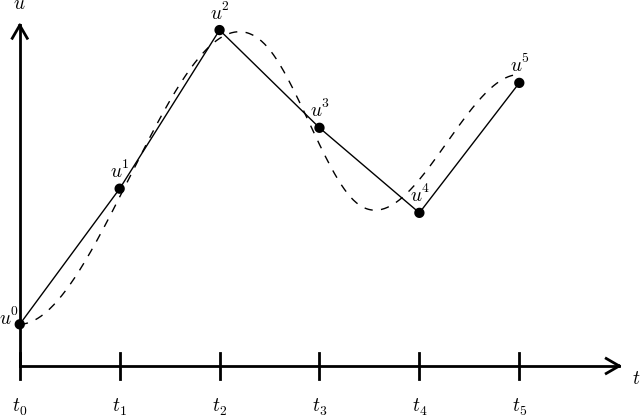
\includegraphics[width=0.7\linewidth]{fig-alg/fdm_u_uei.png}}




\end{frame}

\begin{frame}[plain,fragile]
\frametitle{Topics in the first intro to the finite difference method}

\begin{block}{Contents }
\begin{itemize}
 \item How to think about finite difference discretization

 \item Key concepts:
\begin{itemize}

   \item mesh

   \item mesh function

   \item finite difference approximations

\end{itemize}

\noindent
 \item The Forward Euler, Backward Euler, and Crank-Nicolson methods

 \item Finite difference operator notation

 \item How to derive an algorithm and implement it in Python

 \item How to test the implementation
\end{itemize}

\noindent
\end{block}
\end{frame}

\begin{frame}[plain,fragile]
\frametitle{A basic model for exponential decay}

\label{decay:model}

\index{decay (problem)} \index{exponential decay}

The world's simplest (?) ODE:

\begin{equation*}
u'(t) = -au(t),\quad u(0)=I,\ t\in (0,T]
\end{equation*}

\begin{block}{Observation }
We can learn a lot about numerical methods, computer implementation,
program testing, and real applications of these tools by using
this very simple ODE as example. The teaching principle is to keep the math as
simple as possible while learning computer tools.
\end{block}



% inline figure
\centerline{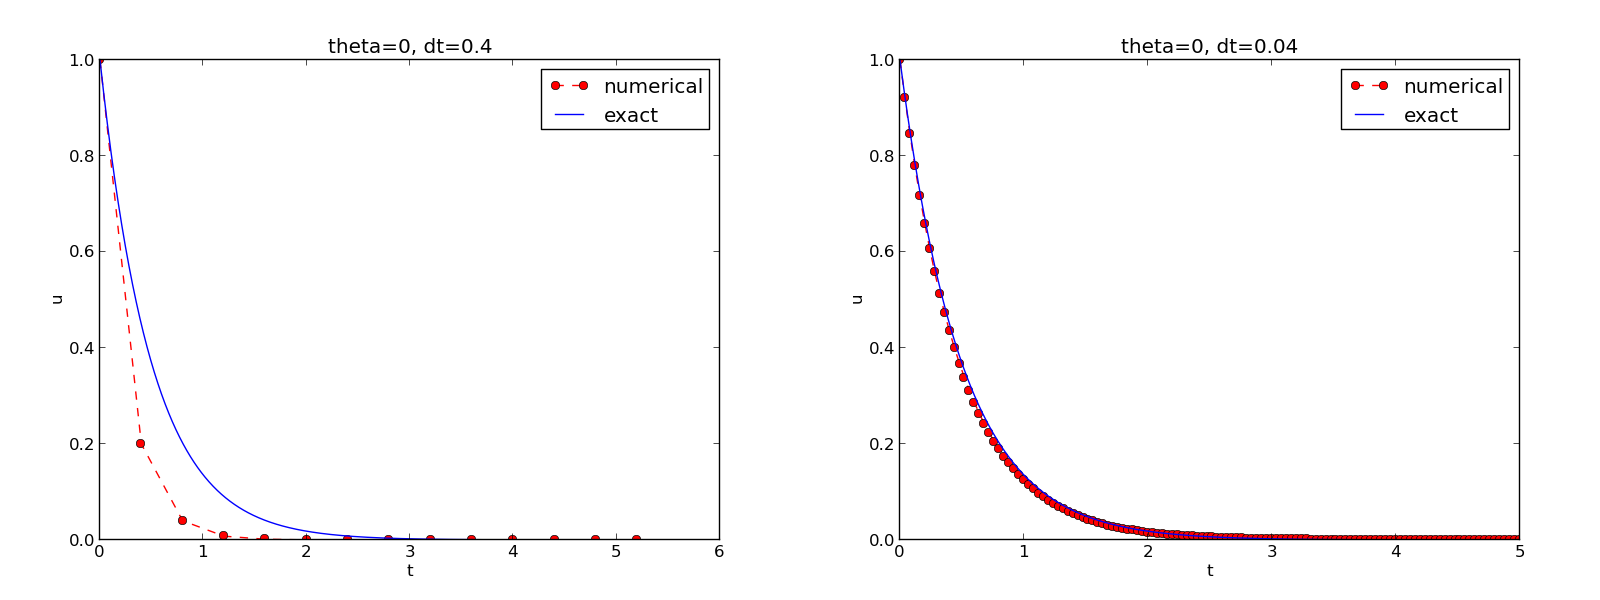
\includegraphics[width=0.7\linewidth]{fig-alg/FE1.png}}
\end{frame}

\begin{frame}[plain,fragile]
\frametitle{The ODE model has a range of applications in many fields}

\begin{itemize}
 \item Growth and decay of populations (cells, animals, human)

 \item Growth and decay of a fortune

 \item Radioactive decay

 \item Cooling/heating of an object

 \item Pressure variation in the atmosphere

 \item Vertical motion of a body in water/air

 \item Time-discretization of diffusion PDEs by Fourier techniques
\end{itemize}

\noindent
See the \href{{http://tinyurl.com/nclmcng/pub/sphinx-decay/._main_decay008.html}}{text} for details.
\end{frame}

\begin{frame}[plain,fragile]
\frametitle{The ODE problem has a continuous and discrete version}

\noindent\textbf{Continuous problem.}
\begin{equation}
u' = -au,\ t\in (0,T], \quad u(0)=I
\label{decay:problem}
\end{equation}
(varies with a continuous $t$)

\noindent\textbf{Discrete problem.}
Numerical methods applied to the continuous problem turns it into
a discrete problem

\begin{equation}
u^{n+1} = \mbox{const} u^n, \quad n=0,1,\ldots N_t-1, \quad u^n=I
\label{decay:problem:discrete}
\end{equation}
(varies with discrete mesh points $t_n$)
\end{frame}

\begin{frame}[plain,fragile]
\frametitle{The steps in the finite difference method}

\label{decay:schemes:keysteps}

Solving a differential equation by a finite difference method
consists of four steps:

\begin{enumerate}
\item discretizing the domain,

\item fulfilling the equation at discrete time points,

\item replacing derivatives by finite differences,

\item formulating a recursive algorithm.
\end{enumerate}

\noindent
\end{frame}

\begin{frame}[plain,fragile]
\frametitle{Step 1: Discretizing the domain}

\index{mesh} \index{grid}


The time domain $[0,T]$ is represented by a \emph{mesh}: a finite number of
$N_t+1$ points

\[0 = t_0 < t_1 < t_2 < \cdots < t_{N_t-1} < t_{N_t} = T\]

\index{mesh function}

\begin{itemize}
 \item We seek the solution $u$ at the mesh points: $u(t_n)$, $n=1,2,\ldots,N_t$.

 \item Note: $u^0$ is known as $I$.

 \item Notational short-form for the numerical approximation to $u(t_n)$: $u^n$

 \item In the differential equation: $u$ is the exact solution

 \item In the numerical method and implementation: $u^n$ is the numerical
   approximation, $\uex(t)$ is the exact solution
\end{itemize}

\noindent
\end{frame}

\begin{frame}[plain,fragile]
\frametitle{Step 1: Discretizing the domain}

$u^n$ is a mesh function, defined at the mesh points $t_n$, $n=0,\ldots,N_t$
only.




% inline figure
\centerline{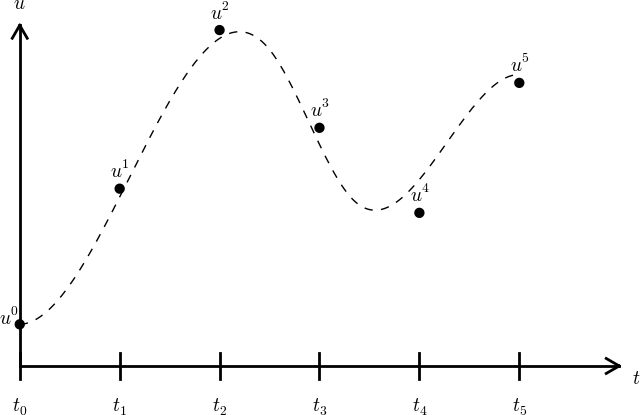
\includegraphics[width=0.7\linewidth]{fig-alg/fdm_u_ue.png}}
\end{frame}

\begin{frame}[plain,fragile]
\frametitle{What about a mesh function between the mesh points?}

Can extend the mesh function to yield values between mesh points
by \emph{linear interpolation}:

\begin{equation}
u(t) \approx u^n + \frac{u^{n+1}-u^n}{t_{n+1}-t_n}(t - t_n)
\end{equation}



% inline figure
\centerline{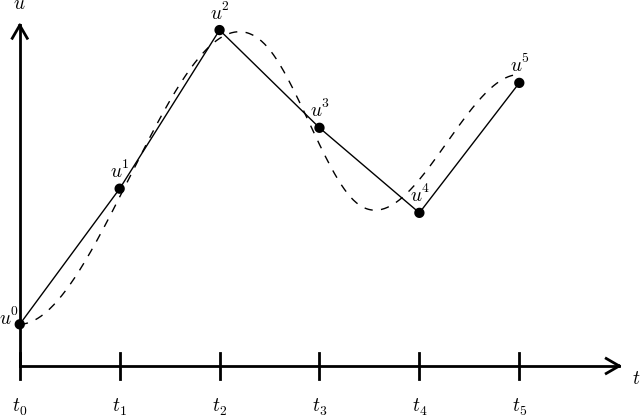
\includegraphics[width=0.7\linewidth]{fig-alg/fdm_u_uei.png}}
\end{frame}

\begin{frame}[plain,fragile]
\frametitle{Step 2: Fulfilling the equation at discrete time points}

\begin{itemize}
 \item The ODE holds for all $t\in (0,T]$ (infinite no of points)

 \item Idea: let the ODE be valid at the mesh points only (finite no of points)
\end{itemize}

\noindent
\begin{equation}
u'(t_n) = -au(t_n),\quad n=1,\ldots,N_t
\label{decay:step2}
\end{equation}

\index{finite differences}
\end{frame}

\begin{frame}[plain,fragile]
\frametitle{Step 3: Replacing derivatives by finite differences}

Now it is time for the \emph{finite difference} approximations of
derivatives:

\begin{equation}
u'(t_n) \approx \frac{u^{n+1}-u^{n}}{t_{n+1}-t_n}
\label{decay:FEdiff}
\end{equation}



% inline figure
\centerline{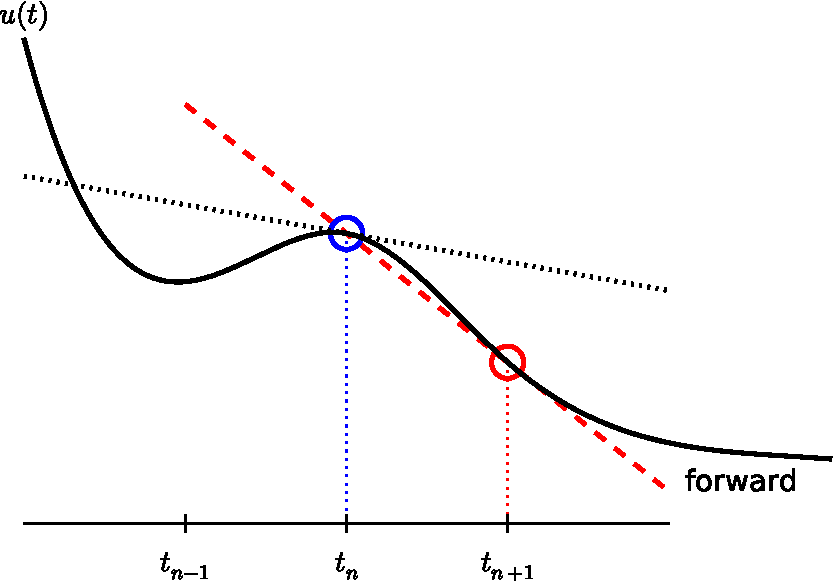
\includegraphics[width=0.8\linewidth]{fig-alg/fd_forward.pdf}}
\end{frame}

\begin{frame}[plain,fragile]
\frametitle{Step 3: Replacing derivatives by finite differences}

Inserting the finite difference approximation in

\[ u'(t_n) = -au(t_n)\]
gives

\begin{equation}
\frac{u^{n+1}-u^{n}}{t_{n+1}-t_n} = -au^{n},\quad n=0,1,\ldots,N_t-1
\label{decay:step3}
\end{equation}

(Known as \emph{discrete equation}, or \emph{discrete problem},
or \emph{finite difference method/scheme})
\end{frame}

\begin{frame}[plain,fragile]
\frametitle{Step 4: Formulating a recursive algorithm}

\index{difference equation}
\index{discrete equation}
\index{algebraic equation}
\index{finite difference scheme}
\index{Forward Euler scheme}

How can we actually compute the $u^n$ values?

\begin{itemize}
  \item given $u^0=I$

  \item compute $u^1$ from $u^0$

  \item compute $u^2$ from $u^1$

  \item compute $u^3$ from $u^2$ (and so forth)
\end{itemize}

\noindent
In general: we have $u^n$ and seek $u^{n+1}$

\begin{block}{The Forward Euler scheme }
Solve wrt $u^{n+1}$ to get the computational formula:

\begin{equation}
u^{n+1} = u^n - a(t_{n+1} -t_n)u^n
\label{decay:FE}
\end{equation}
\end{block}
\end{frame}

\begin{frame}[plain,fragile]
\frametitle{Let us apply the scheme by hand}

Assume constant time spacing: $\Delta t = t_{n+1}-t_n=\mbox{const}$

\begin{align*}
u_0 &= I,\\ 
u_1 & = u^0 - a\Delta t u^0 = I(1-a\Delta t),\\ 
u_2 & = I(1-a\Delta t)^2,\\ 
u^3 &= I(1-a\Delta t)^3,\\ 
&\vdots\\ 
u^{N_t} &= I(1-a\Delta t)^{N_t}
\end{align*}

Ooops - we can find the numerical solution by hand (in this simple
example)! No need for a computer (yet)...
\end{frame}

\begin{frame}[plain,fragile]
\frametitle{A backward difference}

Here is another finite difference approximation to the
derivative (backward difference):

\begin{equation}
u'(t_n) \approx \frac{u^{n}-u^{n-1}}{t_{n}-t_{n-1}}
\label{decay:BEdiff}
\end{equation}



% inline figure
\centerline{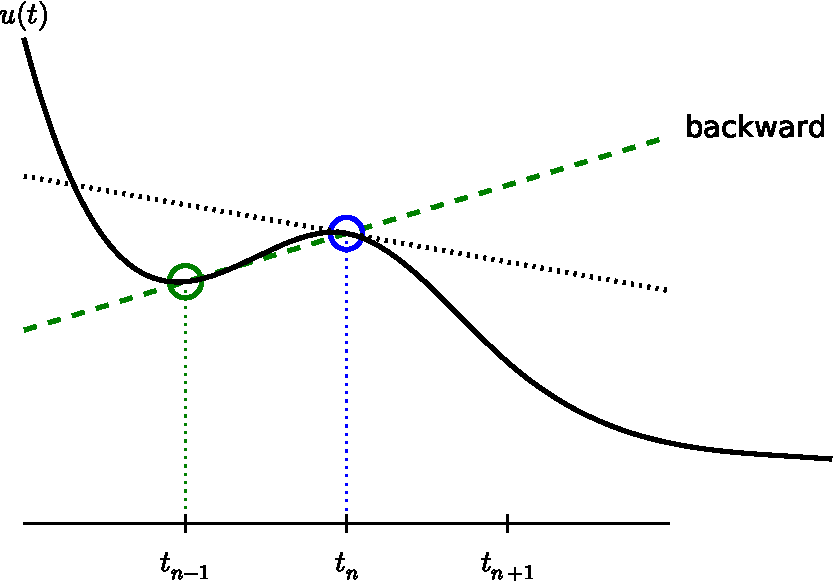
\includegraphics[width=0.8\linewidth]{fig-alg/fd_backward.pdf}}
\end{frame}

\begin{frame}[plain,fragile]
\frametitle{The Backward Euler scheme}

\index{backward scheme, 1-step}
\index{Backward Euler scheme}

Inserting the finite difference approximation in $u'(t_n)=-au(t_n)$ yields
the Backward Euler (BE) scheme:

\begin{equation}
\frac{u^{n}-u^{n-1}}{t_{n}-t_{n-1}} = -a u^n
\label{decay:BE0}
\end{equation}
Solve with respect to the unknown $u^{n+1}$:

\begin{equation}
u^{n+1} = \frac{1}{1+ a(t_{n+1}-t_n)} u^n
\label{decay:BE}
\end{equation}
\end{frame}

\begin{frame}[plain,fragile]
\frametitle{A centered difference}

Centered differences are better approximations than forward or
backward differences.



% inline figure
\centerline{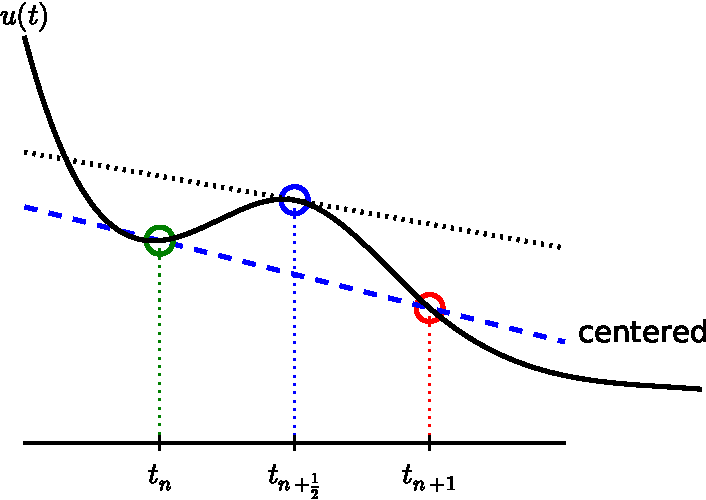
\includegraphics[width=0.8\linewidth]{fig-alg/fd_centered_CN.pdf}}
\end{frame}

\begin{frame}[plain,fragile]
\frametitle{The Crank-Nicolson scheme; ideas}

\label{decay:schemes:CN}

\index{Crank-Nicolson scheme}

Idea 1: let the ODE hold at $t_{n+\half}$

\[ u'(t_{n+\half}) = -au(t_{n+\half})\]

Idea 2: approximate $u'(t_{n+\half}$ by a centered difference

\begin{equation}
u'(t_{n+\half}) \approx \frac{u^{n+1}-u^n}{t_{n+1}-t_n}
\label{decay:CNdiff}
\end{equation}

Problem: $u(t_{n+\half})$ is not defined, only $u^n=u(t_n)$ and $u^{n+1}=u(t_{n+1})$

Solution:

\[ u(t_{n+\half}) \approx \half(u^n + u^{n+1}) \]
\end{frame}

\begin{frame}[plain,fragile]
\frametitle{The Crank-Nicolson scheme; result}

Result:

\begin{equation}
\frac{u^{n+1}-u^n}{t_{n+1}-t_n} = -a\half (u^n + u^{n+1})
\label{decay:CN1}
\end{equation}

Solve wrt to $u^{n+1}$:

\begin{equation}
u^{n+1} = \frac{1-\half a(t_{n+1}-t_n)}{1 + \half a(t_{n+1}-t_n)}u^n
\label{decay:CN}
\end{equation}
This is a Crank-Nicolson (CN) scheme or a midpoint or centered scheme.
\end{frame}

\begin{frame}[plain,fragile]
\frametitle{The unifying $\theta$-rule}

\label{decay:schemes:theta}

\index{weighted average} \index{theta-rule} \index{$\theta$-rule}

The Forward Euler, Backward Euler, and Crank-Nicolson schemes can be
formulated as one scheme with a varying parameter $\theta$:

\begin{equation}
\frac{u^{n+1}-u^{n}}{t_{n+1}-t_n} = -a (\theta u^{n+1} + (1-\theta) u^{n})
\label{decay:th0}
\end{equation}

\begin{itemize}
 \item $\theta =0$: Forward Euler

 \item $\theta =1$: Backward Euler

 \item $\theta =1/2$: Crank-Nicolson

 \item We may alternatively choose any $\theta\in [0,1]$.
\end{itemize}

\noindent
$u^n$ is known, solve for $u^{n+1}$:

\begin{equation}
u^{n+1} = \frac{1 - (1-\theta) a(t_{n+1}-t_n)}{1 + \theta a(t_{n+1}-t_n)}
\label{decay:th}
\end{equation}
\end{frame}

\begin{frame}[plain,fragile]
\frametitle{Constant time step}

Very common assumption (not important, but exclusively used for
simplicity hereafter): constant time step $t_{n+1}-t_n\equiv\Delta t$


\begin{block}{Summary of schemes for constant time step }
\begin{alignat}{2}
u^{n+1} &= (1 - a\Delta t )u^n  & \hbox{Forward Euler}
\label{decay:FE:u}\\ 
u^{n+1} &= \frac{1}{1+ a\Delta t} u^n  & \hbox{Backward Euler}
\label{decay:BE:u}\\ 
u^{n+1} &= \frac{1-\half a\Delta t}{1 + \half a\Delta t} u^n & \hbox{Crank-Nicolson}
\label{decay:CN:u}\\ 
u^{n+1} &= \frac{1 - (1-\theta) a\Delta t}{1 + \theta a \Delta t}u^n  & \hbox{The }\theta-\hbox{rule}
\label{decay:th:u}
\end{alignat}
\end{block}
\end{frame}

\begin{frame}[plain,fragile]
\frametitle{Test the understanding!}

Derive Forward Euler, Backward Euler, and Crank-Nicolson schemes for
Newton's law of cooling:

\[ T' = -k(T-T_s),\quad T(0)=T_0,\ t\in (0,t_{\mbox{end}}]\]

Physical quantities:

\begin{itemize}
 \item $T(t)$: temperature of an object at time $t$

 \item $k$: parameter expressing heat loss to the surroundings

 \item $T_s$: temperature of the surroundings

 \item $T_0$: initial temperature
\end{itemize}

\noindent
\end{frame}

\begin{frame}[plain,fragile]
\frametitle{Compact operator notation for finite differences}

\label{decay:fd:op}

\index{finite difference operator notation} \index{operator notation, finite differences}

\begin{itemize}
 \item Finite difference formulas can be tedious to write and read/understand

 \item Handy tool: finite difference operator notation

 \item Advantage: communicates the nature of the difference in a compact way
\end{itemize}

\noindent
\begin{equation}
[D_t^- u  = -au]^n
\end{equation}
\end{frame}

\begin{frame}[plain,fragile]
\frametitle{Specific notation for difference operators}

Forward difference:

\begin{equation}
[D_t^+u]^n = \frac{u^{n+1} - u^{n}}{\Delta t}
\approx \frac{d}{dt} u(t_n) \label{fd:D:f}
\end{equation}
Centered difference:

\begin{equation}
[D_tu]^n = \frac{u^{n+\half} - u^{n-\half}}{\Delta t}
\approx \frac{d}{dt} u(t_n), \label{fd:D:c}
\end{equation}

Backward difference:
\begin{equation}
[D_t^-u]^n = \frac{u^{n} - u^{n-1}}{\Delta t}
\approx \frac{d}{dt} u(t_n) \label{fd:D:b}
\end{equation}
\end{frame}

\begin{frame}[plain,fragile]
\frametitle{The Backward Euler scheme with operator notation}

\begin{equation*}
[D_t^-u]^n = -au^n
\end{equation*}

Common to put the whole equation inside square brackets:

\begin{equation}
[D_t^- u  = -au]^n
\end{equation}
\end{frame}

\begin{frame}[plain,fragile]
\frametitle{The Forward Euler scheme with operator notation}

\begin{equation}
[D_t^+ u  = -au]^n
\end{equation}
\end{frame}

\begin{frame}[plain,fragile]
\frametitle{The Crank-Nicolson scheme with operator notation}

Introduce an averaging operator:

\begin{equation}
[\overline{u}^{t}]^n = \half (u^{n-\half} + u^{n+\half} )
\approx u(t_n) \label{fd:mean:a}
\end{equation}

The Crank-Nicolson scheme can then be written as

\begin{equation}
[D_t u = -a\overline{u}^t]^{n+\half}
\label{fd:compact:ex:CN}
\end{equation}

Test: use the definitions and write out the above formula to see that
it really is the Crank-Nicolson scheme!
\end{frame}

\section{Implementation}

\begin{frame}[plain,fragile]
\frametitle{Implementation}

\label{decay:impl1}

Model:
\[
u'(t) = -au(t),\quad t\in (0,T], \quad u(0)=I
\]

Numerical method:

\[
u^{n+1} = \frac{1 - (1-\theta) a\Delta t}{1 + \theta a\Delta t}u^n
\]
for $\theta\in [0,1]$. Note

\begin{itemize}
 \item $\theta=0$ gives Forward Euler

 \item $\theta=1$ gives Backward Euler

 \item $\theta=1/2$ gives Crank-Nicolson
\end{itemize}

\noindent

\end{frame}

\begin{frame}[plain,fragile]
\frametitle{Requirements of a program}

\begin{itemize}
  \item Compute the numerical solution $u^n$, $n=1,2,\ldots,N_t$

  \item Display the numerical and exact solution $\uex(t)=e^{-at}$

  \item Bring evidence to a correct implementation (\emph{verification})

  \item Compare the numerical and the exact solution in a plot

  \item computes the error $\uex (t_n) - u^n$

  \item computes the convergence rate of the numerical scheme

  \item reads its input data from the command line
\end{itemize}

\noindent
\end{frame}

\begin{frame}[plain,fragile]
\frametitle{Tools to learn}

\begin{itemize}
  \item Basic \href{{http://python.org}}{Python} programming

  \item Array computing with \href{{http://numpy.org/}}{\nolinkurl{numpy}}

  \item Plotting with \href{{http://matplotlib.sourceforge.net/}}{\nolinkurl{matplotlib.pyplot}} and \href{{https://github.com/hplgit/scitools/}}{\nolinkurl{scitools}}

  \item File writing and reading
\end{itemize}

\noindent
\begin{block}{Notice}
All programs are in the directory
\href{{http://tinyurl.com/ofkw6kc/alg}}{\nolinkurl{src/alg}}.
\end{block}
\end{frame}

\begin{frame}[plain,fragile]
\frametitle{Why implement in Python?}

\begin{itemize}
  \item Python has a very clean, readable syntax (often known as
    "executable pseudo-code").

  \item Python code is very similar to MATLAB code (and MATLAB has a
    particularly widespread use for scientific computing).

  \item Python is a full-fledged, very powerful programming language.

  \item Python is similar to, but much simpler to work with and
    results in more reliable code than C++.
\end{itemize}

\noindent
\end{frame}

\begin{frame}[plain,fragile]
\frametitle{Why implement in Python?}

\begin{itemize}
  \item Python has a rich set of modules for scientific computing, and its
    popularity in scientific computing is rapidly growing.

  \item Python was made for being combined with compiled languages
    (C, C++, Fortran) to reuse existing numerical software and to
    reach high computational performance of new implementations.

  \item Python has extensive support for administrative task
    needed when doing large-scale computational investigations.

  \item Python has extensive support for graphics (visualization,
    user interfaces, web applications).

  \item FEniCS, a very powerful tool for solving PDEs by
    the finite element method, is most human-efficient to operate
    from Python.
\end{itemize}

\noindent
\end{frame}

\begin{frame}[plain,fragile]
\frametitle{Algorithm}

\label{decay:py1}

\begin{itemize}
 \item Store $u^n$, $n=0,1,\ldots,N_t$ in an array \texttt{u}.

 \item Algorithm:
\begin{enumerate}

  \item initialize $u^0$

  \item for $t=t_n$, $n=1,2,\ldots,N_t$: compute $u_n$ using
     the $\theta$-rule formula
\end{enumerate}

\noindent
\end{itemize}

\noindent
\end{frame}

\begin{frame}[plain,fragile]
\frametitle{Translation to Python function}

\begin{minted}[fontsize=\fontsize{9pt}{9pt},linenos=false,mathescape,baselinestretch=1.0,fontfamily=tt,xleftmargin=2mm]{python}
from numpy import *

def solver(I, a, T, dt, theta):
    """Solve u'=-a*u, u(0)=I, for t in (0,T] with steps of dt."""
    Nt = int(T/dt)            # no of time intervals
    T = Nt*dt                 # adjust T to fit time step dt
    u = zeros(Nt+1)           # array of u[n] values
    t = linspace(0, T, Nt+1)  # time mesh

    u[0] = I                  # assign initial condition
    for n in range(0, Nt):    # n=0,1,...,Nt-1
        u[n+1] = (1 - (1-theta)*a*dt)/(1 + theta*dt*a)*u[n]
    return u, t
\end{minted}

Note about the \texttt{for} loop: \texttt{range(0, Nt, s)} generates all integers
from \texttt{0} to \texttt{Nt} in steps of \texttt{s} (default 1), \emph{but not including} \texttt{Nt} (!).

Sample call:
\begin{minted}[fontsize=\fontsize{9pt}{9pt},linenos=false,mathescape,baselinestretch=1.0,fontfamily=tt,xleftmargin=2mm]{python}
u, t = solver(I=1, a=2, T=8, dt=0.8, theta=1)
\end{minted}
\end{frame}

\begin{frame}[plain,fragile]
\frametitle{Integer division}

Python applies integer division: \texttt{1/2} is 0, while \texttt{1./2} or \texttt{1.0/2} or
\texttt{1/2.} or \texttt{1/2.0} or \texttt{1.0/2.0} all give 0.5.

A safer \texttt{solver} function (\texttt{dt = float(dt)} - guarantee float):

\begin{minted}[fontsize=\fontsize{9pt}{9pt},linenos=false,mathescape,baselinestretch=1.0,fontfamily=tt,xleftmargin=2mm]{python}
from numpy import *

def solver(I, a, T, dt, theta):
    """Solve u'=-a*u, u(0)=I, for t in (0,T] with steps of dt."""
    dt = float(dt)            # avoid integer division
    Nt = int(round(T/dt))     # no of time intervals
    T = Nt*dt                 # adjust T to fit time step dt
    u = zeros(Nt+1)           # array of u[n] values
    t = linspace(0, T, Nt+1)  # time mesh

    u[0] = I                  # assign initial condition
    for n in range(0, Nt):    # n=0,1,...,Nt-1
        u[n+1] = (1 - (1-theta)*a*dt)/(1 + theta*dt*a)*u[n]
    return u, t
\end{minted}
\end{frame}

\begin{frame}[plain,fragile]
\frametitle{Doc strings}

\begin{itemize}
 \item First string after the function heading

 \item Used for documenting the function

 \item Automatic documentation tools can make fancy manuals for you

 \item Can be used for automatic testing
\end{itemize}

\noindent
\begin{minted}[fontsize=\fontsize{9pt}{9pt},linenos=false,mathescape,baselinestretch=1.0,fontfamily=tt,xleftmargin=2mm]{python}
def solver(I, a, T, dt, theta):
    """
    Solve

        u'(t) = -a*u(t),

    with initial condition u(0)=I, for t in the time interval
    (0,T]. The time interval is divided into time steps of
    length dt.

    theta=1 corresponds to the Backward Euler scheme, theta=0
    to the Forward Euler scheme, and theta=0.5 to the Crank-
    Nicolson method.
    """
    ...
\end{minted}
\end{frame}

\begin{frame}[plain,fragile]
\frametitle{Formatting of numbers}

Can control formatting of reals and integers through the \emph{printf} format:

\begin{minted}[fontsize=\fontsize{9pt}{9pt},linenos=false,mathescape,baselinestretch=1.0,fontfamily=tt,xleftmargin=2mm]{python}
print 't=%6.3f u=%g' % (t[i], u[i])
\end{minted}

Or the alternative \emph{format string syntax}:
\begin{minted}[fontsize=\fontsize{9pt}{9pt},linenos=false,mathescape,baselinestretch=1.0,fontfamily=tt,xleftmargin=2mm]{python}
print 't={t:6.3f} u={u:g}'.format(t=t[i], u=u[i])
\end{minted}
\end{frame}

\begin{frame}[plain,fragile]
\frametitle{Running the program}

How to run the program \href{{http://tinyurl.com/ofkw6kc/alg/decay_v1.py}}{\nolinkurl{decay_v1.py}}.

\begin{minted}[fontsize=\fontsize{9pt}{9pt},linenos=false,mathescape,baselinestretch=1.0,fontfamily=tt,xleftmargin=2mm]{console}
Terminal> python decay_v1.py
\end{minted}

Can also run it as "normal" Unix programs: \Verb!./decay_v1.py! if the
first line is

\begin{minted}[fontsize=\fontsize{9pt}{9pt},linenos=false,mathescape,baselinestretch=1.0,fontfamily=tt,xleftmargin=2mm]{python}
`#!/usr/bin/env python`
\end{minted}

Then
\begin{minted}[fontsize=\fontsize{9pt}{9pt},linenos=false,mathescape,baselinestretch=1.0,fontfamily=tt,xleftmargin=2mm]{console}
Terminal> chmod a+rx decay_v1.py
Terminal> ./decay_v1.py
\end{minted}
\end{frame}

\begin{frame}[plain,fragile]
\frametitle{Plotting the solution}

Basic syntax:

\begin{minted}[fontsize=\fontsize{9pt}{9pt},linenos=false,mathescape,baselinestretch=1.0,fontfamily=tt,xleftmargin=2mm]{python}
from matplotlib.pyplot import *

plot(t, u)
show()
\end{minted}

Can (and should!) add labels on axes, title, legends.
\end{frame}

\begin{frame}[plain,fragile]
\frametitle{Comparing with the exact solution}

Python function for the exact solution $\uex(t)=Ie^{-at}$:

\begin{minted}[fontsize=\fontsize{9pt}{9pt},linenos=false,mathescape,baselinestretch=1.0,fontfamily=tt,xleftmargin=2mm]{python}
def u_exact(t, I, a):
    return I*exp(-a*t)
\end{minted}

Quick plotting:

\begin{minted}[fontsize=\fontsize{9pt}{9pt},linenos=false,mathescape,baselinestretch=1.0,fontfamily=tt,xleftmargin=2mm]{python}
u_e = u_exact(t, I, a)
plot(t, u, t, u_e)
\end{minted}

Problem: $\uex(t)$ applies the same mesh as $u^n$ and
looks as a piecewise linear function.

Remedy: Introduce a very fine mesh for $\uex$.

\begin{minted}[fontsize=\fontsize{9pt}{9pt},linenos=false,mathescape,baselinestretch=1.0,fontfamily=tt,xleftmargin=2mm]{python}
t_e = linspace(0, T, 1001)      # fine mesh
u_e = u_exact(t_e, I, a)

plot(t_e, u_e, 'b-',            # blue line for u_e
     t,   u,   'r--o')          # red dashes w/circles
\end{minted}
\end{frame}

\begin{frame}[plain,fragile]
\frametitle{Add legends, axes labels, title, and wrap in a function}

\begin{minted}[fontsize=\fontsize{9pt}{9pt},linenos=false,mathescape,baselinestretch=1.0,fontfamily=tt,xleftmargin=2mm]{python}
from matplotlib.pyplot import *

def plot_numerical_and_exact(theta, I, a, T, dt):
    """Compare the numerical and exact solution in a plot."""
    u, t = solver(I=I, a=a, T=T, dt=dt, theta=theta)

    t_e = linspace(0, T, 1001)        # fine mesh for u_e
    u_e = u_exact(t_e, I, a)

    plot(t,   u,   'r--o',            # red dashes w/circles
         t_e, u_e, 'b-')              # blue line for exact sol.
    legend(['numerical', 'exact'])
    xlabel('t')
    ylabel('u')
    title('theta=%g, dt=%g' % (theta, dt))
    savefig('plot_%s_%g.png' % (theta, dt))
\end{minted}

Complete code in
\href{{http://tinyurl.com/ofkw6kc/alg/decay_v2.py}}{\nolinkurl{decay_v2.py}}



% inline figure
\centerline{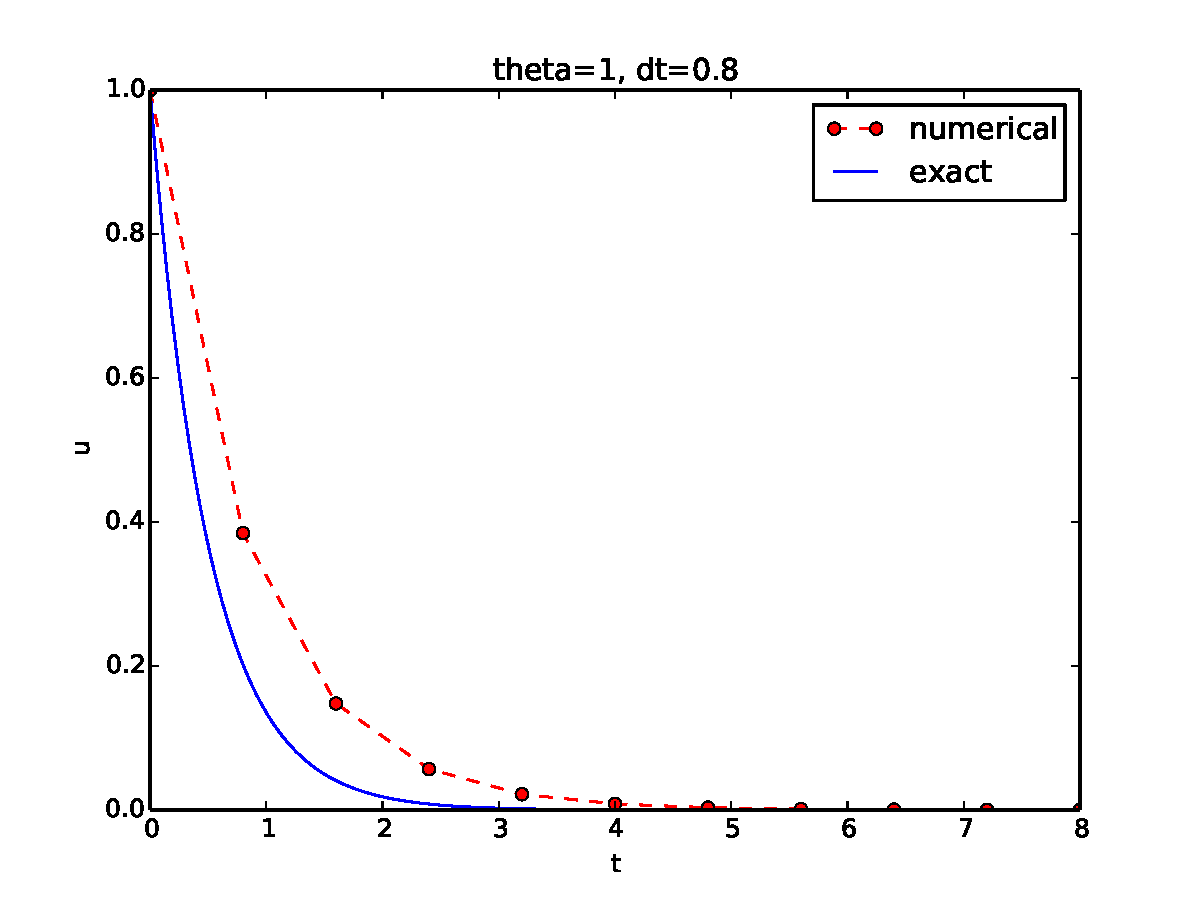
\includegraphics[width=0.8\linewidth]{fig-alg/decay_v2.pdf}}
\end{frame}

\begin{frame}[plain,fragile]
\frametitle{Plotting with SciTools}

\href{{https://github.com/hplgit/scitools}}{SciTools} provides a
unified plotting interface (Easyviz) to many different plotting
packages: Matplotlib, Gnuplot, Grace, VTK, OpenDX, ...

Can use Matplotlib (MATLAB-like) syntax,
or a more compact \texttt{plot} function syntax:

\begin{minted}[fontsize=\fontsize{9pt}{9pt},linenos=false,mathescape,baselinestretch=1.0,fontfamily=tt,xleftmargin=2mm]{python}
from scitools.std import *

plot(t,   u,   'r--o',           # red dashes w/circles
     t_e, u_e, 'b-',             # blue line for exact sol.
     legend=['numerical', 'exact'],
     xlabel='t',
     ylabel='u',
     title='theta=%g, dt=%g' % (theta, dt),
     savefig='%s_%g.png' % (theta2name[theta], dt),
     show=True)
\end{minted}

Change backend (plotting engine, Matplotlib by default):

\begin{minted}[fontsize=\fontsize{9pt}{9pt},linenos=false,mathescape,baselinestretch=1.0,fontfamily=tt,xleftmargin=2mm]{console}
Terminal> python decay_plot_st.py --SCITOOLS_easyviz_backend gnuplot
Terminal> python decay_plot_st.py --SCITOOLS_easyviz_backend grace
\end{minted}
\end{frame}

\section{Verifying the implementation}

\begin{frame}[plain,fragile]
\frametitle{Verifying the implementation}

\label{decay:verification}


\begin{itemize}
 \item Verification = bring evidence that the program works

 \item Find suitable test problems

 \item Make function for each test problem

 \item Later: put the verification tests in a professional testing framework
\end{itemize}

\noindent

\end{frame}

\begin{frame}[plain,fragile]
\frametitle{Simplest method: run a few algorithmic steps by hand}

Use a calculator ($I=0.1$, $\theta=0.8$, $\Delta t =0.8$):

\[ A\equiv \frac{1 - (1-\theta) a\Delta t}{1 + \theta a \Delta t} = 0.298245614035\]

\begin{align*}
u^1 &= AI=0.0298245614035,\\ 
u^2 &= Au^1= 0.00889504462912,\\ 
u^3 &=Au^2= 0.00265290804728
\end{align*}

See the function \Verb!verify_three_steps! in \href{{http://tinyurl.com/ofkw6kc/alg/decay_verf1.py}}{\nolinkurl{decay_verf1.py}}.
\end{frame}

\begin{frame}[plain,fragile]
\frametitle{Comparison with an exact discrete solution}

\begin{block}{Best verification }
Compare computed numerical solution
with a closed-form \emph{exact discrete solution} (if possible).
\end{block}

Define
\[ A = \frac{1 - (1-\theta) a\Delta t}{1 + \theta a \Delta t}\]
Repeated use of the $\theta$-rule:
\begin{align*}
u^0 &= I,\\ 
u^1 &= Au^0 = AI\\ 
u^n &= A^nu^{n-1} = A^nI
\end{align*}
\end{frame}

\begin{frame}[plain,fragile]
\frametitle{Making a test based on an exact discrete solution}

The exact discrete solution is

\begin{equation}
u^n = IA^n
\label{decay:un:exact}
\end{equation}

\begin{block}{Question}
Understand what $n$ in $u^n$ and in $A^n$ means!
\end{block}

Test if

\[ \max_n |u^n - \uex(t_n)| < \epsilon\sim 10^{-15}\]

Implementation in \href{{http://tinyurl.com/ofkw6kc/alg/decay_verf2.py}}{\nolinkurl{decay_verf2.py}}.
\end{frame}

\begin{frame}[plain,fragile]
\frametitle{Test the understanding!}

Make a program for solving Newton's law of cooling

\[ T' = -k(T-T_s),\quad T(0)=T_0,\ t\in (0,t_{\mbox{end}}]\]
with the Forward Euler, Backward Euler, and Crank-Nicolson schemes
(or a $\theta$ scheme). Verify the implementation.
\end{frame}

\begin{frame}[plain,fragile]
\frametitle{Computing the numerical error as a mesh function}

\label{decay:computing:error}

Task: compute the numerical error $e^n = \uex(t_n) - u^n$

Exact solution: $\uex(t)=Ie^{-at}$, implemented as

\begin{minted}[fontsize=\fontsize{9pt}{9pt},linenos=false,mathescape,baselinestretch=1.0,fontfamily=tt,xleftmargin=2mm]{python}
def u_exact(t, I, a):
    return I*exp(-a*t)
\end{minted}

Compute $e^n$ by

\begin{minted}[fontsize=\fontsize{9pt}{9pt},linenos=false,mathescape,baselinestretch=1.0,fontfamily=tt,xleftmargin=2mm]{python}
u, t = solver(I, a, T, dt, theta)  # Numerical solution
u_e = u_exact(t, I, a)
e = u_e - u
\end{minted}

\begin{block}{Array arithmetics - we compute on entire arrays! }

\begin{itemize}
 \item \Verb!u_exact(t, I, a)! works with \texttt{t} as array

 \item Must have \texttt{exp} from \texttt{numpy} (not \texttt{math})

 \item \Verb!e = u_e - u!: array subtraction

 \item Array arithmetics gives shorter and much faster code
\end{itemize}

\noindent
\end{block}
\end{frame}

\begin{frame}[plain,fragile]
\frametitle{Computing the norm of the error}

\label{decay:computing:error:norm}

\begin{itemize}
 \item $e^n$ is a mesh function

 \item Usually we want one number for the error

 \item Use a norm of $e^n$
\end{itemize}

\noindent
Norms of a function $f(t)$:

\begin{align}
||f||_{L^2} &= \left( \int_0^T f(t)^2 dt\right)^{1/2}
\label{decay:norms:L2}\\ 
||f||_{L^1} &= \int_0^T |f(t)| dt
\label{decay:norms:L1}\\ 
||f||_{L^\infty} &= \max_{t\in [0,T]}|f(t)|
\label{decay:norms:Linf}
\end{align}
\end{frame}

\begin{frame}[plain,fragile]
\frametitle{Norms of mesh functions}

\begin{itemize}
 \item Problem: $f^n =f(t_n)$ is a mesh function and hence not defined for all $t$.
   How to integrate $f^n$?

 \item Idea: Apply a numerical integration rule, using only
   the mesh points of the mesh function.
\end{itemize}

\noindent
The Trapezoidal rule:

\[ ||f^n|| = \left(\Delta t\left(\half(f^0)^2 + \half(f^{N_t})^2
+ \sum_{n=1}^{N_t-1} (f^n)^2\right)\right)^{1/2} \]

Common simplification yields the $L^2$ norm of a mesh function:

\[ ||f^n||_{\ell^2} = \left(\Delta t\sum_{n=0}^{N_t} (f^n)^2\right)^{1/2}\]
\end{frame}

\begin{frame}[plain,fragile]
\frametitle{Implementation of the norm of the error}

\[ E = ||e^n||_{\ell^2}  = \sqrt{\Delta t\sum_{n=0}^{N_t} (e^n)^2}\]

Python w/array arithmetics:

\begin{minted}[fontsize=\fontsize{9pt}{9pt},linenos=false,mathescape,baselinestretch=1.0,fontfamily=tt,xleftmargin=2mm]{python}
e = u_exact(t) - u
E = sqrt(dt*sum(e**2))
\end{minted}
\end{frame}

\begin{frame}[plain,fragile]
\frametitle{Comment on array vs scalar computation}

Scalar computing of \texttt{E = sqrt(dt*sum(e**2))}:

\begin{minted}[fontsize=\fontsize{9pt}{9pt},linenos=false,mathescape,baselinestretch=1.0,fontfamily=tt,xleftmargin=2mm]{python}
m = len(u)     # length of u array (alt: u.size)
u_e = zeros(m)
t = 0
for i in range(m):
    u_e[i] = u_exact(t, a, I)
    t = t + dt
e = zeros(m)
for i in range(m):
    e[i] = u_e[i] - u[i]
s = 0  # summation variable
for i in range(m):
    s = s + e[i]**2
error = sqrt(dt*s)
\end{minted}
Obviously, scalar computing

\begin{itemize}
 \item takes more code

 \item is less readable

 \item runs much slower
\end{itemize}

\noindent
\begin{block}{Rule }
Compute on entire arrays (when possible)!
\end{block}
\end{frame}

\begin{frame}[plain,fragile]
\frametitle{Memory-saving implementation}

\begin{itemize}
 \item Note 1: we store the entire array \texttt{u}, i.e., $u^n$ for $n=0,1,\ldots,N_t$

 \item Note 2: the formula for $u^{n+1}$ needs $u^n$ only, not $u^{n-1}$, $u^{n-2}$, ...

 \item No need to store more than $u^{n+1}$ and $u^{n}$

 \item Extremely important when solving PDEs

 \item No practical importance here (much memory available)

 \item But let's illustrate how to do save memory!

 \item Idea 1: store $u^{n+1}$ in \texttt{u}, $u^n$ in \Verb!u_1! (\texttt{float})

 \item Idea 2: store \texttt{u} in a file, read file later for plotting
\end{itemize}

\noindent
\end{frame}

\begin{frame}[plain,fragile]
\frametitle{Memory-saving solver function}

\begin{minted}[fontsize=\fontsize{9pt}{9pt},linenos=false,mathescape,baselinestretch=1.0,fontfamily=tt,xleftmargin=2mm]{python}
def solver_memsave(I, a, T, dt, theta, filename='sol.dat'):
    """
    Solve u'=-a*u, u(0)=I, for t in (0,T] with steps of dt.
    Minimum use of memory. The solution is stored in a file
    (with name filename) for later plotting.
    """
    dt = float(dt)         # avoid integer division
    Nt = int(round(T/dt))  # no of intervals

    outfile = open(filename, 'w')
    # u: time level n+1, u_1: time level n
    t = 0
    u_1 = I
    outfile.write('%.16E  %.16E\n' % (t, u_1))
    for n in range(1, Nt+1):
        u = (1 - (1-theta)*a*dt)/(1 + theta*dt*a)*u_1
        u_1 = u
        t += dt
        outfile.write('%.16E  %.16E\n' % (t, u))
    outfile.close()
    return u, t
\end{minted}
\end{frame}

\begin{frame}[plain,fragile]
\frametitle{Reading computed data from file}

\begin{minted}[fontsize=\fontsize{9pt}{9pt},linenos=false,mathescape,baselinestretch=1.0,fontfamily=tt,xleftmargin=2mm]{python}
def read_file(filename='sol.dat'):
    infile = open(filename, 'r')
    u = [];  t = []
    for line in infile:
        words = line.split()
        if len(words) != 2:
            print 'Found more than two numbers on a line!', words
            sys.exit(1)  # abort
        t.append(float(words[0]))
        u.append(float(words[1]))
    return np.array(t), np.array(u)
\end{minted}

Simpler code with \texttt{numpy} functionality for reading/writing tabular data:

\begin{minted}[fontsize=\fontsize{9pt}{9pt},linenos=false,mathescape,baselinestretch=1.0,fontfamily=tt,xleftmargin=2mm]{python}
def read_file_numpy(filename='sol.dat'):
    data = np.loadtxt(filename)
    t = data[:,0]
    u = data[:,1]
    return t, u
\end{minted}

Similar function \texttt{np.savetxt}, but then we need all $u^n$ and $t^n$ values
in a two-dimensional array (which we try to prevent now!).
\end{frame}

\begin{frame}[plain,fragile]
\frametitle{Usage of memory-saving code}

\begin{minted}[fontsize=\fontsize{9pt}{9pt},linenos=false,mathescape,baselinestretch=1.0,fontfamily=tt,xleftmargin=2mm]{python}
def explore(I, a, T, dt, theta=0.5, makeplot=True):
    filename = 'u.dat'
    u, t = solver_memsave(I, a, T, dt, theta, filename)

    t, u = read_file(filename)
    u_e = u_exact(t, I, a)
    e = u_e - u
    E = np.sqrt(dt*np.sum(e**2))
    if makeplot:
        plt.figure()
        ...
\end{minted}

Complete program: \href{{http://tinyurl.com/ofkw6kc/alg/decay_memsave.py}}{\nolinkurl{decay_memsave.py}}.
\end{frame}

\end{document}
